\documentclass[a4paper,9pt,landscape]{extarticle}
\usepackage{multicol}
\usepackage{calc}
\usepackage{ifthen}
\usepackage[landscape]{geometry}
\usepackage{pgfplots}
\usepgfplotslibrary{fillbetween}

\usepackage{graphicx}
\usepackage{amsmath, amssymb, amsthm}
\DeclareMathOperator*{\argmin}{argmin}
\DeclareMathOperator*{\argmax}{argmax}

\usepackage{latexsym, marvosym}
\usepackage{pifont}
\usepackage{lscape}
\usepackage{dsfont}
\usepackage{graphicx}
\usepackage{array}
\usepackage{booktabs}
\usepackage[bottom]{footmisc}
\usepackage{tikz}
\usetikzlibrary{shapes}
\usepackage{pdfpages}
\usepackage{wrapfig}
\usepackage{enumitem}
\setlist[description]{leftmargin=0pt}
\usepackage{xfrac}
\usepackage[pdftex,
pdfauthor={Janus Advincula},
pdftitle={Probability},
pdfkeywords={probability} {statistics} {cheatsheet} {pdf} {cheat} {sheet} {formulas} {equations}
]{hyperref}
\usepackage[
open,
openlevel=2
]{bookmark}
\usepackage{relsize}
\usepackage{rotating}

\newcommand\independent{\protect\mathpalette{\protect\independenT}{\perp}}
\def\independenT#1#2{\mathrel{\setbox0\hbox{$#1#2$}%
		\copy0\kern-\wd0\mkern4mu\box0}} 

\newcommand{\noin}{\noindent}    
\newcommand{\logit}{\textrm{logit}} 
\newcommand{\var}{\textrm{Var}}
\newcommand{\cov}{\textrm{Cov}} 
\newcommand{\corr}{\textrm{Corr}} 
\newcommand{\N}{\mathcal{N}}
\newcommand{\Bern}{\textrm{Bern}}
\newcommand{\Bin}{\textrm{Bin}}
\newcommand{\Beta}{\textrm{Beta}}
\newcommand{\Gam}{\textrm{Gamma}}
\newcommand{\Expo}{\textrm{Expo}}
\newcommand{\Pois}{\textrm{Pois}}
\newcommand{\Unif}{\textrm{Unif}}
\newcommand{\Geom}{\textrm{Geom}}
\newcommand{\NBin}{\textrm{NBin}}
\newcommand{\Hypergeometric}{\textrm{HGeom}}
\newcommand{\HGeom}{\textrm{HGeom}}
\newcommand{\Mult}{\textrm{Mult}}

\geometry{top=.2in,left=.2in,right=.2in,bottom=.2in}

\pagestyle{empty}
\makeatletter
\renewcommand{\section}{\@startsection{section}{1}{0mm}%
	{-1ex plus -.5ex minus -.2ex}%
	{0.5ex plus .2ex}%x
	{\normalfont\large\bfseries}}
\renewcommand{\subsection}{\@startsection{subsection}{2}{0mm}%
	{-1explus -.5ex minus -.2ex}%
	{0.5ex plus .2ex}%
	{\normalfont\normalsize\bfseries}}
\renewcommand{\subsubsection}{\@startsection{subsubsection}{3}{0mm}%
	{-1ex plus -.5ex minus -.2ex}%
	{1ex plus .2ex}%
	{\normalfont\small\bfseries}}
\makeatother

\setcounter{secnumdepth}{0}

\setlength{\parindent}{0pt}
\setlength{\parskip}{0pt plus 0.5ex}

% -----------------------------------------------------------------------

\usepackage{titlesec}

\titleformat{\section}
{\color{violet}\normalfont\normalsize\bfseries}
{\color{blue}\thesection}{1em}{}
\titleformat{\subsection}
{\color{violet}\normalfont\normalsize\bfseries}
{\color{violet}\thesection}{1em}{}
% Comment out the above 5 lines for black and white

\begin{document}
	
	\raggedright
	\footnotesize
	\begin{multicols*}{3}
		\setlength{\premulticols}{1pt}
		\setlength{\postmulticols}{1pt}
		\setlength{\multicolsep}{1pt}
		\setlength{\columnsep}{2pt}
		
		%%%%%%%%%%%%%%%%%%%%%%%%%%%%%%%%%%%%
		%%% TITLE
		%%%%%%%%%%%%%%%%%%%%%%%%%%%%%%%%%%%%
		
\begin{center}
		{\color{blue} \large{\textbf{Problems in Probability}}} \\
\end{center}

\begin{enumerate}
	\item A pair of jointly continuous random variables, $X$ and $Y$, have a joint probability density function given by
	$$f_{X,Y}(x,y)=
	\begin{cases}
	c,&\text{in the shaded region of the figure below}\\
	0,&\text{elsewhere.}	
	\end{cases}$$
	\begin{center}
	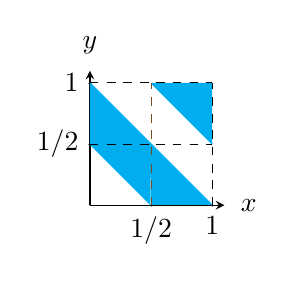
\begin{tikzpicture}[scale=0.3]
	\begin{axis}[every axis plot post/.append style={domain=0:1,samples=100,smooth},
	axis x line = middle,
	axis y line = middle,
	every axis x label/.style={at={(ticklabel* cs:1.05)},anchor=west,},
	every axis y label/.style={at={(ticklabel* cs:1.05)},anchor=south,},
	xtick = {0,0.5,1},
	ytick = {0,0.5,1},
	xticklabels={0,1/2,1},
	yticklabels={0,1/2,1},
	ymax=1.1,
	xmax=1.1,
	xlabel=$x$,
	ylabel=$y$,
	restrict y to domain=0:1,
	axis equal image]
	\addplot[name path=A,domain=0:0.5,cyan]{-x+1/2};
	\addplot[name path=B,domain=0:1,cyan]{-x+1};
	\addplot[name path=C,domain=0.5:1,cyan]{-x+1.5};
	\addplot[name path=D,domain=0:1,dashed]{1.0};
	\addplot[name path=E,domain=0:1,dashed]{0.5};
	\addplot[name path=F,domain=0:1]{0};
	\addplot +[mark=none,dashed] coordinates {(0.5,0) (0.5, 1)};
	\addplot +[mark=none,dashed] coordinates {(1,0) (1, 1)};
	\addplot[cyan] fill between[of=A and B, soft clip={domain=0:0.5}];
	\addplot[cyan] fill between[of=F and B, soft clip={domain=0.5:1}];
	\addplot[cyan] fill between[of=C and D, soft clip={domain=0.5:1}];
	\end{axis}
	\end{tikzpicture}
	\end{center}
	\begin{enumerate}
		\item Find $c$.
		\item Find the marginal PDFs of $X$ and $Y$, i.e., $f_X(x)$ and $f_Y(y)$.
		\item Find $\mathds{E}\left[X|Y=1/4\right]$ and $\var(\left[X|Y=1/4\right])$, that is, the conditional mean and conditional variance of $X$ given that $Y=1/4$.
		\item Find the conditional PDF for $X$ given that $Y=3/4$, i.e., $f_{X|Y}(x|3/4)$.
	\end{enumerate}
	\item Al, Bonnie and Clyde run laps around a track, with the duration of each lap (in hours) being exponentially distributed with parameters $\lambda_A=21$, $\lambda_B=23$, and $\lambda_C=24$, respectively. Assume that all lap durations are independent. At the completion of each lap, a runner drinks either one or two cups of water, with probabilities $1/3$ and $2/3$, respectively, independent of everything else, including how much water was consumed after previous laps. (The time spent drinking is negligible, assumed zero.)
	\begin{enumerate}
		\item Write down the PMF of the total number of completed laps over the first hour.
		\item What is the expected number of cups of water to be consumed by the three runners, in total, over the first hour.
		\item Al has amazing endurance and completed 72 laps. Find a good approximation for the probability that he drank at least 130 cups. (You do not have to use 1/2-corrections.)
		\item What is the probability that Al finishes his first lap before any of the others?
		\item Suppose that the runners have been running for a very long time when you arrive at the track. What is the distribution of the duration of Al's current lap? (This includes the duration of that lap both before and after the time of your arrival.)
		\item Suppose that the runners have been running for $1/4$ hours. What is the distribution of the time Al spends on his second lap, given that he is on his second lap?
	\end{enumerate}
	\item A pulse of light has energy $X$ that is second-order Erlang random variable with parameter $\lambda$, i.e., its PDF is
	\begin{equation}
		f_X(x)=\begin{cases}
		\lambda^2xe^{-\lambda x},&\text{for }x\geq0,\\
		0,&\text{otherwise.}
		\end{cases}
	\end{equation}
	This pulse illuminates an ideal photon-counting detector whose output $N$ is a Poisson-distributed random variable with mean $x$ when $X=x$, i.e., its conditional PMF is
	$$p_{N|X}(n|x)=\begin{cases}
		\dfrac{x^ne^{-x}}{n!},&\text{for }n=0,1,2,\dots,\\
		0,&\text{otherwise.}
	\end{cases}$$
	\begin{enumerate}
		\item Find $\mathds{E}\left[N\right]$ and $\var(N)$, the unconditional mean and variance of $N$.
		\item Find $p_N(n)$, the unconditional PMF of $N$.
		\item Find $\widehat{X}_\text{lin}(N)$, the linear least-squares estimator of $X$ based on an observation of $N$.
		\item Find $\widehat{X}_\text{MAP}(N)$, the MAP estimator of $X$ based on an observation of $N$.
		\item Instead of the prior distribution in Eq. (1), we are now told that
		$$\mathds{P}(X=2)=\frac{3^3}{35},\quad\mathds{P}(X=3)=\frac{2^3}{35}.$$ Given the observation $N=3$, and in order to minimize the probability of error, which one of the two hypotheses $X=2$ and $X=3$ should be chosen?
	\end{enumerate}
	Note: $\int\limits_{0}^{\infty}y^ke^{-\alpha y}dy=\dfrac{k!}{\alpha^{k+1}},$ for $\alpha>0$ and $k=0,1,2,\dots.$
	\item Alice shows up at an Athena cluster at time zero and spends her time exclusively in typing emails. The times that her emails are sent are a Poisson process with rate $\lambda_A$ per hour.
	\begin{enumerate}
		\item What is the probability that Alice sent exactly three emails during the time interval $[1,2]$?
		\item Let $Y_1$ and $Y_2$ be the times at which Alice's first and second emails were sent.
		\begin{enumerate}
			\item Find $\mathds{E}\left[Y_2|Y_1\right]$.
			\item Find the PDF of $Y_1^2$.
			\item Find the joint PDF of $Y_1$ and $Y_2$.
		\end{enumerate}
		\item You show up at time 1 and you are told that Alice has sent exactly one email so far.
		\begin{enumerate}
			\item What is the conditional expectation of $Y_2$ given this information?
			\item What is the conditional expectation of $Y_1$ given this information?
		\end{enumerate}
		\item Bob just finished exercising (without email access) and sits next to Alice at time 1. He starts typing emails at time 1, and fires them according to an independent Poisson process with rate $\lambda_B$.
		\begin{enumerate}
			\item What is the PMF of the total number of emails sent by the two of them together during the interval $[0,2]$?
			\item What is the expected value of the total typing time associated with the email that Alice is typing at the time that Bob shows up? (Here, "total typing time`` includes the time that Alice spent on that email both before and after Bob's arrival.)
			\item What is the expected value of the time until each one of them has sent at least one email? (Note that we count time starting from time 0, and we take into account any emails possibly sent out by Alice during the interval $[0,1]$.)
			\item Given that a total of 10 emails were sent during the interval $[0,2]$, what is the probability that exactly 4 of them were sent by Alice?
		\end{enumerate}
		\item Suppose that $\lambda_A=4$. Use Chebyshev's inequality to find an upper bound on the probability that Alice sent at least 5 emails during the time interval $[0,1]$. Does the Markov inequality provide a better bound?
		\item You do not know $\lambda_A$ but you watch Alice for an hour and see that she sent exactly 5 emails. Derive the maximum likelihood estimate of $\lambda_A$ based on this information.
		\item We have reasons to believe that $\lambda_A$ is a large number. Let $N$ be the number of emails sent during the interval $[0,1]$. Justify why the CLT can be applied to $N$, and give a precise statement of the CLT in this case.
		\item Under the same assumption as in last part, that $\lambda_A$ is large, you can now pretend that $N$ is a normal random variable. Suppose that you observe that value of $N$. Give an (approximately) 95\% confidence interval for $\lambda_A$. State precisely what approximations you are making. {\it Possibly useful facts:} The cumulative normal distribution satisfies $\Phi(1.645)=0.95$ and $\Phi(1.96)=0.975$.
		\item You are now told that $\lambda_A$ is actually the realized value of an exponential random variable $\Lambda$, with parameter 2:
		$$f_\Lambda(\lambda)=2e^{-2\lambda},\quad\lambda\geq0.$$
		\begin{enumerate}
			\item Find $\mathds{E}\left[N^2\right]$.
			\item Find the linear least squares estimator of $\Lambda$ given $N$.
		\end{enumerate}
	\end{enumerate}
	\item Alice and Bob each choose a number independently and uniformly at random from the interval $[0,2]$. Consider the following events:
	
	$A$: The absolute difference between the two numbers is greater than $1/4$.
	
	$B$: Alice's number is greater than $1/4$.
	
	Find $\mathds{P}(A\cap B)$.
	\item There are $m$ red balls and $n$ white balls in an urn. We draw two balls simultaneously and at random. What is the probability that the balls are of different color?
	\item 20 black pebbles are arranged in 4 rows of 5 pebbles each. We choose 4 of these pebbles at random and order them red. What is the probability that all the red pebbles lie in different rows?
	\item We have two light bulbs, A and B. Bulb A has an exponentially distributed lifetime with mean lifetime 4 days. Bulb B has an exponentially distributed lifetime with mean lifetime 6 days. We select one of the two bulbs at random; each bulb is equally likely to be chosen. Given that the bulb we selected is still working after 12 days, what is the probability that we selected bulb A?
	\item A test for some rare disease is assumed to be correct 95\% of the time: if a person has the disease, the test results are positive with probability 0.95., and if the person does not have the disease, the test results are negative with probability 0.95. A random person drawn from a certain population has probability 0.001 of having the disease. Given that the person just tested positive, what is the probability of having the disease?
	\item Let $X$ be a random variable with
	$$f_X(x)=\begin{cases}
		2e^{-2x}&\text{if }x\geq0,\\
		0,&\text{otherwise.}
	\end{cases}$$
	Let $Y=2X-4$. Find $f_Y(0)$.
	\item A number $p$ is drawn from the interval $[0,1]$ according to the uniform distribution, and then a sequence of independent Bernoulli trials is performed, each with success probability $p$. What is the variance of the number of successes in $k$ trials? {\it Note $k$ is a deterministic number.}
	\item A police radar always over-estimates the speed of incoming cars by an amount that is uniformly distributed between 0 and 5 mph. Assume that car speeds are uniformly distributed between 60 and 75 mph and are independent of the radar over-estimate. If the radar measures a speed of 76 mph, what is the least squares estimate of the actual car speed?
	\item You are visiting the Killian rainforest, when you insect repellent runs out. This forest is infested with lethal mosquitoes, whose second bite will kill any human instantaneously. Assume mosquito's land on your back and deliver a vicious bite according to a Bernoulli process. Also assume the expected time till the first bite is 10 seconds. If you arrive at the forest at $t=0$, what is the probability that you die at exactly $t=10$ seconds?
	\item In order to estimate $p$, the fraction of people who will vote for G. Bush in the next election, you conduct a poll of $n$ people drawn randomly and independently from the population. Your estimator $M_n$ iw obtained by dividing $S_n$, the number of people who vote for Bush in your sample, by $n$, i.e., $M_n=S_n/n$. Find the smallest value of $n$, the number of people you must poll, for which the Chebyshev inequality yields a quarantee that
	$$\mathds{P}\left(\left|M_n-p\right|\geq0.01\right)\leq0.01.$$
	(Use the fact that $p(1-p)\leq1/4$ for any $p\in[0,1]$.)
	\item On each day of the year, it rains with probability 0.1, independent of every other day. Use the Central Limit Theorem (CLT) (with no half step) to approximate the probability that, out of the 365 days in a year, it will rain on at least 100 days. Denote the standard normal CDF by $\Phi$.
	\item You take a safari trip to the Porobilati game reserve. A highlight of the game reserve is the Poseni river where one can watch deer and elephants coming to drink water. Deer come to the river according to a Poisson process with arrival rate $\lambda_d=8$ per hour; elephants come to the river according to an independent Poisson process with arrival rate $\lambda_e=2$ per hour. On the first day of your safari, you reach the Poseni river early in the morning hoping to see some elephants. Assume that deer and elephants are the only kinds of animals that visit this river.
	\begin{enumerate}
		\item Let $N$ be the number of animals you see during the first 3 hours. Find $\mathds{E}[N]$ and $\var(N)$.
		\item What's the probability of seeing your 3\textsuperscript{rd} elephant before your 9\textsuperscript{th} deer?
		\item At the end of 3 hours, you have seen 24 deer but no elephants. What is the probability that you will see an elephant in the next hour?
		\item It is now 6 hours since you started watching. You have seen 53 deer but there is still no sight of an elephant. How many more deer do you expect to see before you see your first elephant?
		\item Unfortunately, you forgot your camera in your lodge the first day. You come back with your camera the next day and plan to stay at the river until you've clicked a picture of both a deer and an elephant. Assume you're always able to click a picture as soon as an animal arrives. How long do you expect to stay?
		\item Your friend, a wildlife photographer, is fascinated by the stories of your trip, and decides to take the safari herself. All excited, she arrives at the Poseni river, and is prepared to stay as long as required in order to get lots of beautiful pictures. Unfortunately, she dropped her camera in a bush on the way, as a result of which the camera is not functioning properly; each time she clicks, there is a probability 0.1 that the camera will produce a faulty picture, independently of everything else. Assume she clicks one picture each time an elephant or deer arrives at the river, as soon as it arrives. Let $X$ be the time (in hours) until she gets her third successful picture of an elephant. Find the PDF of $X$.
	\end{enumerate}
	\item Earthquakes in Sumatra occur according to a Poisson process of rate $\lambda=2/$year. Conditioned on the event that exactly two earthquakes take place in a year, what is the probability that both earthquakes occur in the first three months of the year? (For simplicity, assume all months have 30 days, and each year has 12 months, i.e., 360 days.)
	\item Random variables $X$ and $Y$ are such that the pair $(X,Y)$ is uniformly distributed over the trapezoid $A$ with corners $(0,0), (1,2), (3,2)$ and $(4,0)$ shown in the figure:
	\begin{center}
	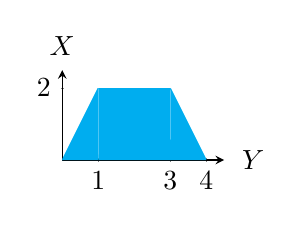
\begin{tikzpicture}[scale=0.3]
	\begin{axis}[every axis plot post/.append style={domain=0:4.2,samples=700,smooth},
	axis x line = middle,
	axis y line = middle,
	every axis x label/.style={at={(ticklabel* cs:1.05)},anchor=west,},
	every axis y label/.style={at={(ticklabel* cs:1.05)},anchor=south,},
	xtick = {1,3,4},
	ytick = {0,2},
	xticklabels={1,3,4},
	yticklabels={0,2},
	ymax=2.5,
	xmax=4.5,
	xlabel=$Y$,
	ylabel=$X$,
	restrict y to domain=0:2,
	axis equal image]
	\addplot[name path=A,domain=0:1,cyan]{2*x};
	\path[name path=axis] (axis cs:0,0) -- (axis cs:4,0);
	\path[name path=axis2] (axis cs:1,2) -- (axis cs:3,2);
	\addplot[name path=C,domain=3:4,cyan]{-2*x+8};
	\addplot[cyan] fill between[of=A and axis, soft clip={domain=0:1}];
	\addplot[cyan] fill between[of=axis2 and axis, soft clip={domain=1:3}];
	\addplot[cyan] fill between[of=C and axis, soft clip={domain=3:4}];
	\end{axis}
	\end{tikzpicture}
	\end{center}
	i.e., $$f_{X,Y}(x,y)=\begin{cases}
		c,&(x,y)\in A\\
		0,&\text{else.}
	\end{cases}$$
	We observe $Y$ and use it to estimate $X$. Let $\widehat{X}$ be the least mean squared error estimator of $X$ given $Y$. What is the value of $\var\left(\widehat{X}-X|Y=1\right)$?
	\item Aliens of two races (blue and green) are arriving on Earth independently according to Poisson process distributions with parameters $\lambda_b$ and $\lambda_g$ respectively. The Alien Arrival Registration Service Authority (AARSA) will begin registering alien arrivals soon.

	Let $T_1$ denote the time AARSA will function until it registers its first alien. Let $G$ be the event that the first alien to be registered is a green one. Let $T_2$ be the time AARSA will function until at least one alien of both races is registered.
	\begin{enumerate}
		\item Express $\mu_1=\mathds{E}[T_1]$ in terms of $\lambda_g$ and $\lambda_b$.
		\item Express $p=\mathds{P}(G)$ in terms of $\lambda_g$ and $\lambda_b$.
		\item Express $\mu_2=\mathds{E}[T_2]$ in terms of $\lambda_g$ and $\lambda_b$.
	\end{enumerate}
	\item Researcher Jill is interested in studying employment in technology firms in Dilicon Valley. She denotes by $X_i$ the number of employees in technology firm $i$ and assumes that $X_i$ are independent and identically distributed with mean $p$. To estimate $p$, Jill randomly interviews $n$ technology firms and observes the number of employees in these firms.
	\begin{enumerate}
		\item Jill uses $$M_n=\frac{X_1+\dots+X_n}{n}$$ as an estimator for $p$. Find the limit of $\mathds{P}(M_n\leq x)$ as $n\rightarrow\infty$ for $x<p$. Find the limit of $\mathds{P}(M_n\leq x)$ as $n\rightarrow\infty$ for $x>p$.
		\item Find the smallest $n$, the number of technology firms Jill must sample, for which the Chebyshev inequality yields a guarantee $$\mathds{P}\left(\left|M_n-p\right|\geq0.5\right)\leq0.05.$$ Assume that $\var(X_i)=v$ for some constant $v$. State your solution as a function of $v$.
		\item Assume now that the researcher samples $n=5000$ firms. Find an approximate value for the probability $$\mathds{P}\left(\left|M_{5000}-p\right|\geq0.5\right)$$
		using the Central Limit Theorem. Assume again that $\var(X_i)=v$ for some constant $v$. Give your answer in terms of $v$, and the standard normal CDF $\Phi$.
	\end{enumerate}
	\item The Random View window factory produces window panes. After manufacturing, 1000 panes were loaded onto a truck. The weight $W_i$ of the $i$\textsuperscript{th} pane (in pounds) on the truck is modeled as a random variable, with the assumption that the $W_i$'s are independent and identically distributed.
	\begin{enumerate}
		\item Assume that the measured weight of the load on the truck was 2340 pounds, and that $\var(W_i)\leq4$. Find an approximate 95 percent confidence interval for $\mu=\mathds{E}[W_i]$, using the Central Limit Theorem.
		\item Now assume instead that the random variables $W_i$ are i.i.d., with an exponential distribution with parameter $\theta>0$, i.e., a distribution with PDF $$f_W(w;\theta)=\theta e^{-\theta w}.$$ What is the maximum likelihood estimate of $\theta$, given that the truckload has weight 2340 pounds?
	\end{enumerate}
	\item A newscast covering the final baseball game between Sed Rox and Y Nakee becomes noisy at the crucial moment when the viewers are informed whether Y Nakee won the game.
	
	Let $a$ be the parameter describing the actual outcome: $a=1$ if Y Nakee won, $a=-1$ otherwise. There were $n$ viewers listening to the telecast. Let $Y_i$ be the information received by viewer $i$ ($1\leq i\leq n$). Under the noisy telecast, $Y_i=a$ with probability $p$, and $Y_i=-a$ with probability $1-p$. Assume that the random variables $Y_i$ are independent of each other.
	
	The vieweres as a group come up with a joint estimator $$Z_n=\begin{cases}
		1&\text{if }\sum_{i=1}^{n}Y_i\geq0,\\
		-1&\text{otherwise.}
	\end{cases}$$
	\begin{enumerate}
		\item Find $\lim\limits_{n\rightarrow\infty}\mathds{P}(Z_n=a)$ assuming that $p>0.5$ and $a=1$.
		\item Find $\lim\limits_{n\rightarrow\infty}\mathds{P}(Z_n=a)$ assuming that $p=0.5$ and $a=1$.
	\end{enumerate}
	\item Let $X,Y,Z$ be three independent (i.e., mutually independent) random variables, each uniformly distributed on the interval $[0,1]$.
	\begin{enumerate}
		\item Find the mean and variance of $\dfrac{1}{Z+1}$.
		\item Find the mean of $\dfrac{XY}{Z+1}$.
		\item Find the probability that $\dfrac{XY}{Z}\leq1$.
	\end{enumerate}
	\item Bob goes to a party, wearing a hat that fits him well. At the end of the party, Bob picks up a hat without looking at it. He knows that the hat he has picked is his own with probability $p$. As a first check to see if he has picked up his own hat, he tries the hat, and if it fits, he decides that it is his own hat.
	
	However, even if the hat picked by Bob is not his own, it is still possible that it fits with probability $q$. Given that Bob picked a hat that fits him, what is the probability that he is correct in deciding that the hat is indeed his own?
	\item For a fixed real number $k>1$, define $c_k=\sum\limits_{i=1}^{\infty}n^{-k}$. Let $X$ and $Y$ be two independent, positive, integer-valued random variables, with $$\mathds{P}(X=n)=\mathds{P}(Y=n)=\dfrac{1}{c_k}n^{-k},\quad\text{for }n=1,2,\dots$$
	Note that the constant $c_k$ is defined to ensure that this PMF sums to 1.
	\begin{enumerate}
		\item Find the probability $\mathds{P}(X=Y)$, in terms of $c_k$.
		\item Fix a positive integer $n$, and define the following event:
		$$A_n\triangleq\{X\text{ is divisible by }n\}.$$
		Find the probability of $A_n$. Your answer should be a function of $n$ and $k$.
	\end{enumerate}
	\item In this problem, you may find it useful to recall the following fact about Poisson random variables. Let $X$ and $Y$ be two independent Poisson random variables, with means $\lambda_1$ and $\lambda_2$, respectively. Then, $X+Y$ is a Poisson random variable with mean $\lambda_1+\lambda_2$. Arguing in a similar way, a Poisson random variable $X$ with parameter $t$, where $t$ is a positive integer, can be thought of as sum of $t$ independent Poisson random variables $X_1,X_2,\dots,X_t$, each of which has mean 1.
	
	Using the information above, and an appropriate limit theorem, evaluate the following limit: $$\lim\limits_{n\rightarrow\infty}\sum_{k>n+\sqrt{n}}^{\infty}\dfrac{e^{-n}n^k}{k!}.$$
	\item We are given a biased coin, where the probability of Heads if $q$. The bias $q$ is itself the realization of a random variable $Q$ which is uniformly distributed on the interval $[0,1]$. We want to estimate the bias of this coin. We flip it 5 times, and define the (observed) random variable $N$ as the number of Heads in this experiment.
	
	Throughout this problem, you may find the following formula useful: For every positive integers $n,k$,
	$$\int_{0}^{1}x^n(1-x)^kdx=\dfrac{n!k!}{(n+k+1)!}.$$
	\begin{enumerate}
		\item Given the observation $N=3$, calculate the posterior distribution of the bias $Q$. That is, find the conditional distribution of $Q$, given $N=3$.
		\item What is the LMS estimate of $Q$, given $N=3$?
		\item What is the resulting conditional mean squared error of the LMS estimator, given $N=3$?
	\end{enumerate}
	\item Let $X$ and $W$ be independent and uniformly distributed on $[-1,1]$. We have given the following facts:
	$$\mathds{E}[X]=\mathds{E}[X^3]=\mathds{E}[X^5]=0$$
	$$\mathds{E}[X^2]=1/3$$
	$$\mathds{E}[X^4]=1/5$$
	Suppose that $$Y=X^3+W.$$
	\begin{enumerate}
		\item Find the LMS estimate of $Y$, given that $X=x$. (Notice we are trying to estimate $Y$ from $X$, not the opposite direction.)
		\item Find the LLMS estimate for $Y$, given that $X=x$.
	\end{enumerate}
	\item Charlie joins a new reading club, from which he receives books to read. Suppose that books arrive as a Poisson process at a rate $\lambda$ of books per week. For each book, the time it takes for Charlie to read it is exponentially distributed with parameter $\mu$; i.e., on average it takes Charlie $1/\mu$ weeks to finish one book. Assume that the reading times for different books are independent, and also independent from the book arrival process.
	
	The problem with Charlie is that he is easily distracted. If he is reading a book when a new book arrives, he immediately turns to read the new one, and only comes back to the older book when he finishes the new book.
	\begin{enumerate}
		\item When Charlie starts a new book, what is the probability that he can finish this book without being interrupted by a new book?
		\item Given that Charlie receives a new book while reading a book, what is the probability that he can finish both books, the new one and the interrupted one, without further interruption?
		\item What is the expected reading time of a book given that it is not interrupted?
	\end{enumerate}
	\item Starting at time $t=0$, cars arrive at a car wash according to a Poisson process with rate of $\lambda$ cars/hour. At any given moment, the car wash is either free or occupied. The car wash is initially free at time $t=0$. If a car arrives at the car wash when it is free, the car is serviced immediately. Service lasts for 1/4 hours, during which the car wash is occupied. If a car arrives at the car wash when it is occupied, the car is denied service and it leaves the car wash.
	\begin{enumerate}
		\item Write down the PMF $p_N(k)$ of $N$, the number of cars arriving at the car wash between times 0 and 3, in terms of $\lambda$ and $k$.
		\item Find the probability that a car is accepted for service given that it arrives at time $t=1/6$.
		\item Find the PDF $f_{T_2}(t)$ of $T_2$, the time until the second serviced car leaves the car wash.
		\item Find the probability that exactly one car is accepted for service between $t=0$ and $t=1$.
	\end{enumerate}
\end{enumerate}

\end{multicols*}
\end{document}
